\documentclass[a4paper]{article}

\usepackage{amsmath}
\usepackage{amssymb}
\usepackage{amsfonts}
\usepackage[style=iso]{datetime2}
\usepackage[explicit]{titlesec}
\usepackage{amsthm}
\usepackage{array}
\usepackage{graphicx}
\usepackage{float}
\usepackage[skip=1em,indent]{parskip}
\usepackage{caption}
\usepackage{hyperref}

\graphicspath{ {./Images/} }

\theoremstyle{definition}
\newtheorem{problem}{Problem}
\newtheorem{definition}{Definition}

\begin{titlepage}
\title{Faulhaber's Formula and its Connection to Discrete Calculus}
\author{Abdul Musthakin}
\date{March 2025}
\end{titlepage}

\renewcommand{\thesection}{\Roman{section}}

\allowdisplaybreaks

\setlength{\parindent}{0pt}

\begin{document}
\maketitle

\section{Prerequisites}

You need very little to understand everything that will be discussed.
A decent number of new concepts will be introduced, but when I do introduce something, I plan on thoroughly explaining it.
The most important `prerequiste' is the ability to understand new things, and to follow simple the simple logic that will be used to go from one equation to another.

Additionally, knowledge of basic calculus (derivatives, integrals, and the relationship between them) would certainly aid in one's appreciation for the results we will derive.
Whilst someone could technically understand everything without it, I do not think that there would be as much value in doing so.
Connections between that which is seemingly unrelated lies at the heart of what I deem to be interesting in mathematics -- which happens to be most things.
There is a very particular beauty in these connections.
The more you know beforehand, the more you have to link new concepts to.

Summation notation is required to be able to read, and by extension, understand, the maths present here.
As it is just shorthand for repeated addition, I do not consider it to be a `new' piece of maths.
You could pick it up via the simple examples given in the introduction, but prior experience is expected.

\section{Introduction}

The formula for the sum of the first $n$ positive integers is something that many people learn fairly early in school.
\begin{equation*}
    \sum_{i=1}^{n} i = 1 + 2 + 3 + \ldots + n = \frac{n(n+1)}{2}
\end{equation*}
The sum of the squares of the first $n$ positive integers, as well as the sum of cubes, have reasonably well-known formulae as well.
\begin{align*}
    \sum_{i=1}^{n} i^2 & = \frac{n(n+1)(2n+1)}{6} \\
    \sum_{i=1}^{n} i^3 & = \frac{n^2 (n+1)^2}{4}
\end{align*}
These formulae are good and all, but how do we prove them?
We can take an algebraic approach, a geometric one, or we may simply use induction.
The latter method will always work as long as we already have an algebraic expression for the sum in terms of $n$.
What if we do not have the end result to prove?
Thus, the problem arises -- deriving a formula for the sum of the $k$-th powers of the first $n$ positive integers: Faulhaber's formula.
\begin{equation*}
    S_k(n) = \sum_{i=1}^{n} i^k = 1^k + 2^k + ... + n^k = \text{ ?}
\end{equation*}
$S_k$ is just another shorthand introduced; the previous three sums can be referred to as $S_1$, $S_2$, and $S_3$.
There are several ways of deriving Faulhaber's formula, and the method that I will use is not the most common one.
Whether it is the ``best" way or not is subjective, but, to me, it is certainly the most interesting.

\section{Necessary Definitions}

First, let us suppose that we have some sequence $a$, the $n$-th element of which is denoted as $a_n$.
Now, let us define the forward difference operator, $\Delta$, as follows.
\begin{equation}
    \Delta_n a_n = a_{n+1} - a_n
\end{equation}
Note that $\Delta$ applies to the sequence $a$, and not to $n$-th element of the sequence.
You could write $\Delta_n a_n$ as $(\Delta a)_n$, which may technically be more correct -- but it is rather cumbersome to use.
This is just a minor detail.

The indefinite sum, or the antidifference, of a sequence can be defined in relation to the forward difference.
\begin{equation}
    \Delta_n \sum_n a_n = a_n
\end{equation}
That is, if $\sum_n a_n = A_n$, then
\begin{equation}
    A_{n+1} - A_n = a_n.
\end{equation}
Now, you may notice that this seems familiar.
Basic knowledge of calculus allows us to spot a connection.
We are dealing with differneces in sums, but not in the way that is present in a regular calculus.
We have ventured into the realm of the discrete, as opposed to the continuous which is much more familiar.

The forward difference is the discrete analogue to the derivative.
Where the latter measures the instantaneous rate of change of a function at some point, the former measures the rate of change of a sequence between two points.
Similarly, the antidifference is the discrete analogue to the antiderivative (indefinite integral).

Just as the fundamental theorem of calculus relates derivatives to integrals, we can construct a discrete version of it which relates forward differences to sums.
\begin{align}
    \Delta_n \sum_{i=n_0}^{n} a_i & = a_{n+1} \label{DFTC1}           \\
    \sum_{i=n_0}^n \Delta_i a_i   & = a_{n+1} - a_{n_0} \label{DFTC2}
\end{align}
The proof of these two states are rather simple, only requiring the use of the definitions we have laid out, and the properties of sums.
The proof of the first statement is as follows.
\begin{align*}
    \Delta_n \sum_{i=n_0}^{n} a_i & = \sum_{i=n_0}^{n+1} a_i - \sum_{i=n_0}^{n} a_i         \\
                                  & = a_{n+1} + \sum_{i=n_0}^{n} a_i - \sum_{i=n_0}^{n} a_i \\
                                  & = a_{n+1} \quad \square
\end{align*}
The proof of the second statement does not require much more work than the first.
\begin{align*}
    \sum_{i=n_0}^n \Delta_i a_i & = \sum_{i=n_0}^n (a_{i+1} - a_i)                                \\
                                & = \sum_{i=n_0}^n a_{i+1} - \sum_{i=n_0}^n a_i                   \\
                                & = \sum_{i=n_0+1}^{n+1} a_i - \sum_{i=n_0}^n a_i                 \\
                                & = a_{n+1} - a_{n_0} + \sum_{i=n_0}^{n} a_i - \sum_{i=n_0}^n a_i \\
                                & = a_{n+1} - a_{n_0} \quad \square
\end{align*}
The relationship between the definite sum and its indefinite counterpart follows from the second statement.
\begin{equation}
    \sum_{i=n_0}^n a_n = \sum_{i=n_0}^n \Delta_n A_n = A_{n+1} - A_{n_0}
\end{equation}
Whilst we will not mention indefinite sums again, I thought that their inclusion here would serve to further illustrate the connection between regular old calculus, and what we have started to formulate.
More connections are to be found as we continue on.

There is just one more definition that needs to be made (kind of).
That is the falling factorial.
There are a few different notations for it, but the notation that I will be using is $x^{\underline{k}}$.
This may be read as ``$x$ to the falling $k$".
You can see the falling factorial as just the regular factorial, but with a specified end point.
\begin{equation}
    x^{\underline{k}} = x(x-1)(x-2)\cdots(x-k+1).
\end{equation}

\section{Formulating a Plan}

What we will do next makes a lot more sense if you see everything we have done so far as creating this discrete version of calculus.
The two most important concepts in calculus, the derivative and the integral, have already been translated over.
However, these two things obviously relate to other topics in maths.
You can find the derivative of any polynomial very easily with the power rule.
It would only make sense for there to be some discrete version of this.
Turns out there is, and it involves the falling factorial.
\begin{align*}
    \Delta_x x^{\underline{k}} & = (x+1)^{\underline{k}} - x^{\underline{k}}                     \\
                               & = (x+1)x(x-1)\cdots(x-k+2) - x(x-1)(x-2)\cdots(x-k+1)           \\
                               & = x(x-1)\cdots(x-k+2) \cdot [(x+1) - (x-k+1)]                   \\
                               & = kx(x-1)\cdots(x-k+2)                                          \\
                               & = kx^{\underline{k-1}} \stepcounter{equation}\tag{\theequation}
\end{align*}
Once again, we have an eerily familiar result.
Well, we best make use of it.
It is important to always be clear on what our goal is.
We have a sum to evaluate, and we have created some tools that resemble familiar concepts in calculus.
If instead of a sum, we had an integral to evaluate, one way of doing so would be to express the integrand (everything inside of the integral) as the derivative of something else.
Using the fact that derives and integrals are the opposite of each other, we could then 'cancel them out' to get our answer.
This is the essence of our method.

The sum of the falling factorial can be derived with what we have.
We simply have to rewrite it in terms of the forward difference of some expression, and then utilise \eqref{DFTC1}.
\begin{align*}
    \sum_{i=1}^n i^{\underline{k}} & = \sum_{i=1}^n \Delta_i \frac{i^{\underline{k+1}}}{k+1}                        \\
                                   & = \frac{(n+1)^{\underline{k+1}}}{k+1} - \frac{{1}^{\underline{k+1}}}{k+1}      \\
                                   & = \frac{(n+1)^{\underline{k+1}}}{k+1} \stepcounter{equation}\tag{\theequation}
\end{align*}
A result we used to simplify our expression above was that $x^{\underline{k}} = 0$ if $k > x$.
This is because $x-k+1$ will be less than or equal to 0 (thus one of the factors in the falling factorial will always be 0).
Since $k +1 > 1$ ($x^{\underline{k}}$ does not make sense otherwise), we were able to apply this.
Now, if we can express any sequence in terms of falling factorials, we can evaluate the sum of that sequence.

\section{Simple Cases}

Let us return to $S_1$, which we already have an expression for and can attempt to derive.
Via the definition of the falling factorial, $i^{\underline{1}}=1$.
Thus, formula for the sum of the first $n$ integers can be derived as follows.
\begin{align*}
    S_1 = \sum_{i=1}^{n} i & = \sum_{i=1}^{n} i^{\underline{1}} \\
                           & = \frac{(n+1)^{\underline{2}}}{2}  \\
                           & = \frac{n(n+1)}{2}
\end{align*}
It works!
We can derive the formula for the sum of the squares of the first $n$ integers.
However, we need to find a way to express $i^2$ in terms of falling factorials first.
\begin{align*}
             & i^{\underline{2}} = i(i-1) = i^2 - i                                \\
    \leadsto & i^2 = i^{\underline{2}} + i = i^{\underline{2}} + i^{\underline{1}}
\end{align*}
The rest of the work simply involves using the ``reverse power rule" and simplifying the expression we get.
\begin{align*}
    S_2 & = \sum_{i=1}^{n} i^2                                                  \\
        & = \sum_{i=1}^{n} \left( i^{\underline{2}} + i^{\underline{1}} \right) \\
        & = \frac{(n+1)^{\underline{3}}}{3} + \frac{(n+1)^{\underline{2}}}{2}   \\
        & = \frac{n(n+1)(n-1)}{3} + \frac{n(n+1)}{2}                            \\
        & = \frac{2n(n+1)(n-1) + 3n(n+1)}{6}                                    \\
        & = \frac{n(n+1)[2(n-1) + 3]}{6}                                        \\
        & = \frac{n(n+1)(2n+1)}{6}
\end{align*}
We can continue this for higher powers.
\begin{align*}
             & i^{\underline{3}} = i(i-1)(i-2) = i^3 - 3i^2 + 2i                                                      \\
    \leadsto & i^3 = i^{\underline{3}} + 3i^2 - 2i = i^{\underline{3}} + 3i^{\underline{2}} + i^{\underline{1}}       \\
    \\
    S_3      & = \sum_{i=1}^n i^3                                                                                     \\                                                                                                     & = (i^{\underline{3}} + 3i^{\underline{2}} + i^{\underline{1}}) \\
             & = \frac{(n+1)^{\underline{4}}}{4} + 3\frac{(n+1)^{\underline{3}}}{3} + \frac{(n+1)^{\underline{2}}}{2} \\
             & = \frac{n(n+1)(n-1)(n-2)}{4} + n(n+1)(n-1) + \frac{n(n+1)}{2}                                          \\
             & = \frac{n(n+1)(n-1)(n-2)}{4} + \frac{4n(n+1)(n-1)}{4} + \frac{2n(n+1)}{4}                              \\
             & = \frac{n(n+1)(n-1)(n-2) + 4n(n+1)(n-1) +2n(n+1)}{4}                                                   \\
             & = \frac{n(n+1)[(n-1)(n-2) + 4(n-1) + 2]}{4}                                                            \\
             & = \frac{n(n+1)(n^2+n)}{4}                                                                              \\
             & = \frac{n^2(n+1)^2}{4}
\end{align*}

\section{Generalisation}

We now have a method to find $S_n$ for any $n$.
The amount of work required would increase with time, but the method is exactly the same.
To generalise what we have done, first notice that expanding the falling factorial gives us a polynomial with certain coefficients.
\begin{align*}
    x^{\underline{1}} & = x                                     \\
    x^{\underline{2}} & = x^2 - x                               \\
    x^{\underline{3}} & = x^3 - 3x^2 + 2x                       \\
    x^{\underline{4}} & = x^{4} - 6 x^3 + 11 x^2 - 6 x          \\
    x^{\underline{5}} & = x^5 - 10 x^4 + 35 x^3 - 50 x^2 + 24 x \\
    \vdots
\end{align*}
When we rearrange these polynomials in order to get $x^k$ in terms of falling factorials, we get equations that resemble polynomials.
\begin{align*}
    x   & = x^{\underline{1}}                                                                                          \\
    x^2 & = x^{\underline{2}} + x^{\underline{1}}                                                                      \\
    x^3 & = x^{\underline{3}} + 3 x^{\underline{2}} + x^{\underline{1}}                                                \\
    x^4 & = x^{\underline{4}} + 6 x^{\underline{3}} + 7 x^{\underline{2}} + x^{\underline{1}}                          \\
    x^5 & = x^{\underline{5}} + 10 x^{\underline{4}} + 25 x^{\underline{3}} + 15 x^{\underline{2}} + x^{\underline{1}} \\
    \vdots
\end{align*}
This is the final thing we need.
We can now evaluate $S_n$, because we can express it in terms of a sum of falling factorials.
There is just one problem: those coefficients.
They are called the Stirling numbers of the second kind, denoted as $S(k, i)$ or $k\brace i$, and they can be defined via the above expansion.
\begin{equation}
    x^k = \sum_{i=1}^k {k\brace i} x^{\underline{i}}
\end{equation}
For example,
\begin{equation*}
    x^5 = {5\brace 5} x^{\underline{5}} + {5\brace 4} x^{\underline{4}} + {5\brace 4} x^{\underline{3}} + {5\brace 3} x^{\underline{2}} + {5\brace 1} x^{\underline{1}}.
\end{equation*}
So far, that might feel a bit unsatisfying -- understandably so.
We had some coefficients we wanted to know more about (specifically how to calculate them in general), and we just gave them a name.
How does one actually go about calculating $k\brace i$?

An explicit formula exists, but it is fairly complicated, and there would not be much value in mentioning it without going through its own derivation.
Fortunately, we have recurrence formulae to work with.
Before we start deriving that, note that all $x^k$ can be expressed as the following.
\begin{equation*}
    x^k = \cdots + {k\brace k+2}x^{\underline{k+2}} + {k\brace k+1}x^{\underline{k+1}} + {k\brace k}x^{\underline{k}} + \cdots + {k\brace 1}x^{\underline{1}} + {k\brace 0}x^{\underline{0}}
\end{equation*}
I have just expanded out the definition above, whilst introducing a few extra terms.
This is just to show that it is valid to do so, but any term with $k \brace i$, where $i > k$, equals zero.
Additionally, ${k \brace 0} = 0$ for all k, as can be seen by the absence of a $x^{\underline{0}}$ term in any of our above exapnsions.

With that out of the way, note the following.
\begin{equation*}
    x \cdot x^{\underline{k}} = x^{\underline{k}}(x-k) + kx^{\underline{k}} = x^{\underline{k+1}} + kx^{\underline{k}}
\end{equation*}
Using the definition of the Stirling numbers of the second kind, we have:
\begin{align*}
    x^{k+1} & =x\cdot x^k                                                                                         \\
            & = x \sum_{i=1}^{k} {k\brace i} x^{\underline{i}}                                                    \\
            & =\sum_{i=1}^{k} {k\brace i} x^{\underline{i+1}}+ \sum_{i=1}^{k} i{k\brace i} x^{\underline{i}}      \\
            & = \sum_{i=2}^{k+1} {k\brace i-1} x^{\underline{i}}+ \sum_{i=1}^{k} i{k\brace i} x^{\underline{i}}   \\
            & = \sum_{i=1}^{k+1} {k\brace i-1} x^{\underline{i}}+ \sum_{i=1}^{k+1} i{k\brace i} x^{\underline{i}} \\
            & = \sum_{i=1}^{k+1} \left({k\brace i-1} + i{k\brace i} \right)x^{\underline{i}}.
\end{align*}
We can express $x^{k+1}$ using a more direct approach.
\begin{equation*}
    x^{k+1} = \sum_{i=1}^{k+1} {{k+1}\brace {i}} x^{\underline{i}}
\end{equation*}
We can equate these two results to arrive at our recurrence formula.
\begin{align*}
    \sum_{i=1}^{k+1} {{k+1}\brace {i}} x^{\underline{i}} & = \sum_{i=1}^{k+1} \left({k\brace i-1} + i{k\brace i} \right)x^{\underline{i}} \\
    {{k+1}\brace {i}} x^{\underline{i}}                  & ={k\brace i-1} + i{k\brace i} \stepcounter{equation}\tag{\theequation}
\end{align*}
With this formula, and some initial values -- which we have -- we can find any Stirling number!
An arduous process, sure, but certainly not more than working with incraesingly long polynomials.

Now, we finally have everything we need.
Faulhaber's formula is ready to be presented in all its glory.
The sum of the $k$-th powers of the first $n$ positive integers can be written in terms of the Stirling numbers of the second kind and falling factorials.
\begin{align*}
    S_k & = \sum_{i=1}^n i^k                                                                              \\
        & = \sum_{i=1}^n \sum_{j=1}^k {k\brace j} i^{\underline{j}}                                       \\
        & = \sum_{j=1}^k {k\brace j} \sum_{i=1}^n i^{\underline{j}}      & \text{(Swapped order of sums)} \\
        & = \sum_{j=1}^k {k\brace j} \frac{(n+1)^{\underline{j+1}}}{j+1}
\end{align*}
With a swap of index variables, we get Faulhaber's formula.
\begin{equation}
    S_k = \sum_{i=1}^n i^k = \sum_{i=1}^k {k\brace i} \frac{(n+1)^{\underline{i+1}}}{i+1}
\end{equation}

\section{Conclusion and Additional Remarks}

WIP
They can also be defined as the number of ways to partion a set of $k$ elements into $i$ nonempty subsets.
This representation of $4\brace 1$ to $f\brace 4$ are shown below.
Each colour is its own subset and dots that are not within a colour are within their own subset.
$4\brace 1$ is on the top of the diagram and $4\brace 4$ is on the bottom.

\begin{figure}[H]
    \centering
    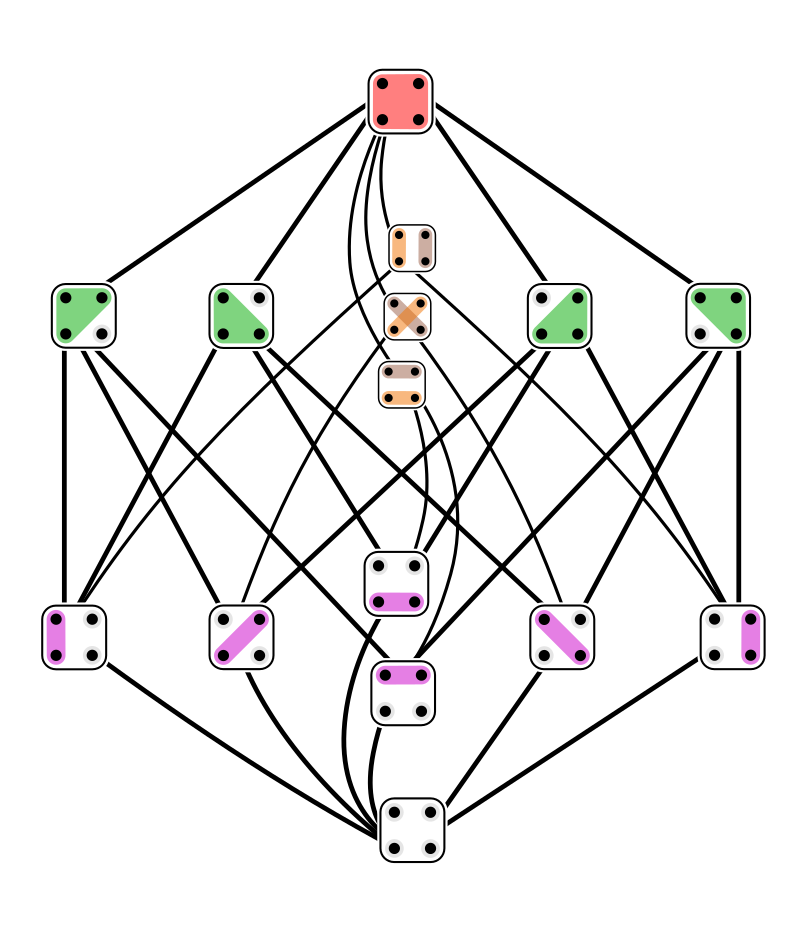
\includegraphics[width=8cm, keepaspectratio]{hasse_diagram.png}
    \captionsetup{justification=centering}
    \caption{Combinatorial Interpretation of S(4, i) Shown in a Hasse Diagram
        \\(Credits: Tilman Piesk, \href{https://creativecommons.org/licenses/by/3.0/}{CC BY 3.0}, via Wikimedia Commons)}
    \label{fig:fig1}
\end{figure}

\end{document}